\DiaryEntry{Quicksort}{2020-01-15}{Algorithms}

The quicksort algorithm is a sorting algorithm and has a worst-case performance of $\Oc(n^2)$ for an input array of length $n$. Its expected average complexity is $\Oc(n \log n)$.

This entry follows Cormen, Introduction to Algorithms.

\subsection{Principle}

The principle of the algorithm is as follows:

\begin{itemize}
  \item Select a pivot element (simplest choice is the last element of the array).
  \item Partition the array into two (posible empty) subarrays: One holding all element smaller or equal than the pivot, the other one holding all elements larger than the pivot.
  \item Process the two subarrays by recursively performing quicksort on them.
\end{itemize}

A Julia implementation following above description looks like this (stored \href{https://github.com/ClemensFMN/JuliaStuff/blob/master/algorithms/quicksort.jl}{here}):

\begin{verbatim}
function quicksort_func(A)
    if(length(A) == 0)
        return A
    else
        pivot = A[end]
        left = filter(x -> x <= pivot, A[1:end-1])
        right = filter(x -> x > pivot, A[1:end-1])
        return [quicksort_func(left) ; [pivot] ; quicksort_func(right)]
    end
end
\end{verbatim}

This is nice, but requires a lot of space as new arrays are created in each recursion. A better implementation needs to perform the partition in-place (by exchanging element in a suitable manner) and returns an index $q$ which separates the two arrays. Using this partition function, a quicksort implementation looks like this.

\begin{verbatim}
function quicksort(A)
   if p<r
      q = parition(A,p,r)
      quicksort(A,p,q-1)
      quicksort(A,q+1,r)
end
\end{verbatim}


\subsection{Partitioning Implementation}

The following scheme performs the partitioning in-place; i.e. no additional space is required. It works with a pointer which separates the two partitions and another pointer wich separates the (upper) partition from the array not yet processed.

The algorithm is as follows

\begin{verbatim}
1 partition(A,p,r)
2   x = A[r]
3   i = p-1
4   for j = p to r-1
5      if A[j] <= x
6         i = i+1
7         exchange A[i] with A[j]
8 exchange A[i+1] with A[r]
9 return i+1
\end{verbatim}

It selects the last element as pivot and, as the routine runs, it partitions the array into four (possibly empty) regions. These are shown in the following Figure.

\begin{figure}[hbt!]
\centering
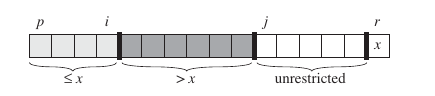
\includegraphics[scale=0.7]{images/quicksort_1.png}
\end{figure}

The region between $p$ and $i$ contains elements already processed and which are smaller or equal than the pivot at position $r$ and being equal to $x$. The region between $i+1$ and $j-1$ contains elements already processed and which are larger than the pivot. Elements between $j$ and $r-1$ have not yet been processed by the procedure.

\paragraph{Algorithm.} The algorithm runs from left to right; the currently processed element is A[j]. If it is smaller than the pivot x, we make more space in the lighlty shaded region (i.e. the region holding elements smaller than the pivot) by incrementing i and move A[i+1] into this region by 
by exchanging A[i+1] with A[j]. Moving the element A[i+1] to its new position is ok, as it larger than the pivot and stays within the correct region.

This case is shown in the following Figure.

\begin{figure}[hbt!]
\centering
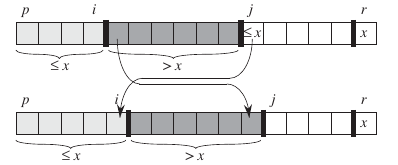
\includegraphics[scale=0.7]{images/quicksort_3.png}
\end{figure}


If the currently processed element A[j] is larger than the pivot we do nothing; j will be increased in the next iteration and thereby correctly reflect the increase of the region holding elements larger than the pivot.

This case is shown in the following Figure.

\begin{figure}[hbt!]
\centering
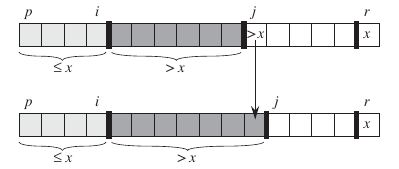
\includegraphics[scale=0.7]{images/quicksort_2.png}
\end{figure}


We are finished when we have processed all elements but the last (the pivot). In the last step we exchange the pivot with the element A[i+1]; this puts the pivot in the right region, the element A[i+1] stays in the region with elements being larger than the pivot.

\paragraph{Example.}

The following example (from Cormen) shows the algorithm in action.

\begin{description}
\item[a] The algorithm starts. Pivot $x = 4$, index $i=0$, and $p=1$ and we process index $j=1$ with $A[j]=2 < x$. Therefore, we exchange $A[j]$ with itself and increase $i$ to $1$. So the region with elements smaller than the pivot has size one; the region with elements larger than the pivot has size zero.

\item[b] We consider element $A[j=2]=8 > x$ and do nothing. By the next increase of $j$ the region of elements larger than the pivot becomes $1$.

\item[c] Similarly, $A[j=3]=7 > x$ and we do nothing.

\item[d] Element $A[j=4]=1 \leq x$, therefore we exchange it with the first element of the region with elements larger than the pivot, $8$.
  
\item[e] Element $A[j=4]=3 \leq x$, and same procedure as in (d).

\item[f] Similarly, $A[j=5]=5 > x$ and we do nothing.

\item[g] Similarly, $A[j=6]=5 > x$ and we do nothing.

\item[h] We are done, as we have processed all elements but the pivot.

\item[i] In the last step, we exchange the pivot with the first element of the region with elements larger than the pivot.

\end{description}

\begin{figure}[hbt!]
\centering
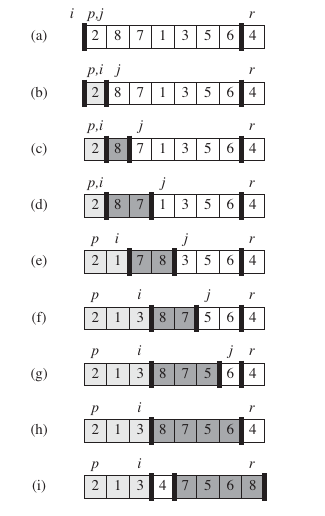
\includegraphics[scale=0.5]{images/quicksort_4.png}
\end{figure}



%%% Local Variables:
%%% mode: latex
%%% TeX-master: "journal"
%%% End:
